\section{Disjoint sr-paths}
\label{section:dpsr}

In the previous section we talked about the general problem of finding sets of disjoint paths over a network.
However, the paths found by these algorithms can be arbitrary and thus hard to implement with segment 
routing as we will show shortly.

In this section we redefine the problem in terms of segment routing and adapt the MIP models from
the previous section accordingly. We start by defining what disjoint sr-path are and the problem of finding
a maximum cardinality set of sr-paths.

\begin{definition}
Let $G$ be a network and $\sr{p}, \sr{q}$ be two sr-paths on $G$. We say that $\sr{p}$ and $\sr{q}$ are \emph{disjoint} if
$E(\sr{p}) \cap E(\sr{q}) = \emptyset$. 
\end{definition}

\begin{problem}{Maximum edge-disjoint sr-paths problem}
\label{prob:max-sr-edp}
\textbf{Input:} A network $G$, two nodes $s, t \in V(G)$ and $k \in \mathbb{N}$.

\textbf{Output:} A set of sr-paths $\{ \sr{p}_1, \ldots, \sr{p}_n \} \subseteq \Pk(s, t)$ such that for each $i \neq j$, $\sr{p}_i$ and $\sr{p}_j$
are disjoint and $n$ is maximum.
\end{problem}

Recall that in case of ECMP between two consecutive segments of $\sr{p}$, the set $E(\sr{p})$ contains the edges belonging to \emph{all} 
those ECMP paths. In other words, we are requiring all those shortest paths corresponding to $\sr{p}$ and $\sr{q}$ to be edge-disjoint.
This is necessary because we can never be sure where exactly the traffic will flow when using a sr-path. In this way, we ensure that no matter how traffic is routed
over ECMPs, no edge will carry packets from two distinct sr-paths $\sr{p}_i$ and $\sr{p}_j$. Figure \ref{fig:non-disjoint} illustrates this with source node $\node{a}$
and destination node $\node{h}$. The two sr-paths displayed
on it are not disjoint because there might both use edge $(\node{e}, \node{h})$ in the event of the green one using path 
$(\edge{a}{c}, \edge{c}{d}, \edge{d}{e}, \edge{e}{h})$ and the blue one using $(\edge{a}{b}, \edge{b}{e}, \edge{e}{h})$.
This can be prevented by, for instance, forcing the blue path to pass thought node $\node{f}$ as shown in Figure \ref{fig:disjoint}.

\begin{figure}
\begin{center}
\begin{tikzpicture}
\def\x{0}
\def\y{0}

\node[scale=0.15] (a) at (0.5 + \x,  0.5 + \y) {\router{a}{router}};
\node[scale=0.15] (b) at (0.5 + \x, -1.0 + \y) {\router{b}{router}};
\node[scale=0.15] (c) at (2.5 + \x,  0.0 + \y) {\router{c}{router}};
\node[scale=0.15] (d) at (4.5 + \x,  0.0 + \y) {\router{d}{router}};
\node[scale=0.15] (e) at (4.0 + \x, -2.0 + \y) {\router{e}{router}};
\node[scale=0.15] (g) at (6.0 + \x,  0.5 + \y) {\router{g}{router}};
\node[scale=0.15] (i) at (8.0 + \x,  0.0 + \y) {\router{i}{router}};
\node[scale=0.15] (h) at (7.0 + \x, -1.5 + \y) {\router{h}{router}};
\node[scale=0.15] (f) at (4.0 + \x, -3.5 + \y) {\router{f}{router}};
\node[scale=0.15] (j) at (8.0 + \x, -2.5 + \y) {\router{j}{router}};
\draw[line width=2] (a) edge[above, sloped] node[black] {} (b);
\draw[line width=2]  (a) edge[above, sloped] node[black] {} (c);

\draw[line width=2] (b) edge[above, sloped] node[black] {} (c);
\draw[line width=2] (b) edge[above, sloped] node[black] {} (e);
\draw[line width=2] (b) edge[above, sloped] node[black] {} (f);
\draw[line width=2]  (c) edge[above, sloped] node[black] {} (d);
\draw[line width=2]  (d) edge[above, sloped] node[black] {} (e);
\draw[line width=2]  (d) edge[above, sloped] node[black] {} (g);
\draw[line width=2] (e) edge[above, sloped] node[black] {} (c);
\draw[line width=2] (e) edge[above, sloped] node[black] {} (f);
\draw[line width=2] (f) edge[above, sloped] node[black] {} (j);
\draw[line width=2] (f) edge[above, sloped] node[black] {} (h);
\draw[line width=2] (g) edge[above, sloped] node[black] {} (i);
\draw[line width=2]  (g) edge[above, sloped] node[black] {} (h);
\draw[line width=2] (h) edge[above, sloped] node[black] {} (j);
\draw[line width=2] (i) edge[above, sloped] node[black] {} (h);
\draw[line width=2, red]  (e) edge[above, sloped] node[black] {} (h);

\draw[line width=3, darkgreen]  (a) edge[above, bend left=15, sloped, ->] node[black] {} (c);
\draw[line width=3, darkgreen]  (c) edge[above, bend left=15, sloped, ->] node[black] {} (d);
\draw[line width=3, darkgreen]  (d) edge[above, bend left=15, sloped, ->] node[black] {} (g);
\draw[line width=3, darkgreen]  (d) edge[above, bend right=15, sloped, ->] node[black] {} (e);
\draw[line width=3, darkgreen]  (e) edge[above, bend left=15, sloped, ->] node[black] {} (h);
\draw[line width=3, darkgreen]  (g) edge[above, bend left=15, sloped, ->] node[black] {} (h);

\draw[line width=3, cyan]  (a) edge[above, bend right=15, sloped, ->] node[black] {} (b);
\draw[line width=3, cyan]  (b) edge[above, bend right=15, sloped, ->] node[black] {} (e);
\draw[line width=3, cyan]  (b) edge[above, bend right=15, sloped, ->] node[black] {} (f);
\draw[line width=3, cyan]  (f) edge[above, bend right=15, sloped, ->] node[black] {} (h);
\draw[line width=3, cyan]  (e) edge[above, bend right=15, sloped, ->] node[black] {} (h);

\node[draw, fill=cyan!20!white, left = 0.1cm of a] (x1) {\small $x_1$};
\node[draw, fill=cyan!20!white, left = 0.1cm of b] (x2) {\small $x_2$};
\node[draw, fill=cyan!20!white, right = 0.1cm of h] (x3) {\small $x_3$};

\node[draw, fill=green!50!white, above = 0.1cm of a] (y1) {\small $y_1$};
\node[draw, fill=green!50!white, above = 0.1cm of d] (y2) {\small $y_2$};
\node[draw, fill=green!50!white, above = 0.1cm of x3] (y3) {\small $y_3$};


\end{tikzpicture}
\end{center}
\caption{The sr-paths $\langle \node{a}, \node{d}, \node{h} \rangle$ and $\langle \node{a}, \node{b}, \node{h} \rangle$ are not edge-disjoint
because their edge sets intersect over $(\node{e}, \node{h})$.}
\label{fig:non-disjoint}
\end{figure}


\begin{figure}
\begin{center}
\begin{tikzpicture}
\def\x{0}
\def\y{0}

\node[scale=0.15] (a) at (0.5 + \x,  0.5 + \y) {\router{a}{router}};
\node[scale=0.15] (b) at (0.5 + \x, -1.0 + \y) {\router{b}{router}};
\node[scale=0.15] (c) at (2.5 + \x,  0.0 + \y) {\router{c}{router}};
\node[scale=0.15] (d) at (4.5 + \x,  0.0 + \y) {\router{d}{router}};
\node[scale=0.15] (e) at (4.0 + \x, -2.0 + \y) {\router{e}{router}};
\node[scale=0.15] (g) at (6.0 + \x,  0.5 + \y) {\router{g}{router}};
\node[scale=0.15] (i) at (8.0 + \x,  0.0 + \y) {\router{i}{router}};
\node[scale=0.15] (h) at (7.0 + \x, -1.5 + \y) {\router{h}{router}};
\node[scale=0.15] (f) at (4.0 + \x, -3.5 + \y) {\router{f}{router}};
\node[scale=0.15] (j) at (8.0 + \x, -2.5 + \y) {\router{j}{router}};
\draw[line width=2] (a) edge[above, sloped] node[black] {} (b);
\draw[line width=2]  (a) edge[above, sloped] node[black] {} (c);

\draw[line width=2] (b) edge[above, sloped] node[black] {} (c);
\draw[line width=2] (b) edge[above, sloped] node[black] {} (e);
\draw[line width=2] (b) edge[above, sloped] node[black] {} (f);
\draw[line width=2]  (c) edge[above, sloped] node[black] {} (d);
\draw[line width=2]  (d) edge[above, sloped] node[black] {} (e);
\draw[line width=2]  (d) edge[above, sloped] node[black] {} (g);
\draw[line width=2] (e) edge[above, sloped] node[black] {} (c);
\draw[line width=2] (e) edge[above, sloped] node[black] {} (f);
\draw[line width=2] (f) edge[above, sloped] node[black] {} (j);
\draw[line width=2] (f) edge[above, sloped] node[black] {} (h);
\draw[line width=2] (g) edge[above, sloped] node[black] {} (i);
\draw[line width=2]  (g) edge[above, sloped] node[black] {} (h);
\draw[line width=2] (h) edge[above, sloped] node[black] {} (j);
\draw[line width=2] (i) edge[above, sloped] node[black] {} (h);
\draw[line width=2]  (e) edge[above, sloped] node[black] {} (h);

\draw[line width=3, darkgreen]  (a) edge[above, bend left=15, sloped, ->] node[black] {} (c);
\draw[line width=3, darkgreen]  (c) edge[above, bend left=15, sloped, ->] node[black] {} (d);
\draw[line width=3, darkgreen]  (d) edge[above, bend left=15, sloped, ->] node[black] {} (g);
\draw[line width=3, darkgreen]  (d) edge[above, bend right=15, sloped, ->] node[black] {} (e);
\draw[line width=3, darkgreen]  (e) edge[above, bend left=15, sloped, ->] node[black] {} (h);
\draw[line width=3, darkgreen]  (g) edge[above, bend left=15, sloped, ->] node[black] {} (h);

\draw[line width=3, cyan]  (a) edge[above, bend right=15, sloped, ->] node[black] {} (b);
\draw[line width=3, cyan]  (b) edge[above, bend right=15, sloped, ->] node[black] {} (f);
\draw[line width=3, cyan]  (f) edge[above, bend right=15, sloped, ->] node[black] {} (h);

\node[draw, fill=cyan!20!white, left = 0.1cm of a] (x1) {\small $x_1$};
\node[draw, fill=cyan!20!white, left = 0.1cm of b] (x2) {\small $x_2$};
\node[draw, fill=cyan!20!white, below = 0.1cm of f] (x3) {\small $x_3$};
\node[draw, fill=cyan!20!white, right = 0.1cm of h] (x4) {\small $x_4$};

\node[draw, fill=green!50!white, above = 0.1cm of a] (y1) {\small $y_1$};
\node[draw, fill=green!50!white, above = 0.1cm of d] (y2) {\small $y_2$};
\node[draw, fill=green!50!white, above = 0.1cm of x4] (y3) {\small $y_3$};


\end{tikzpicture}
\end{center}
\caption{The sr-paths $\langle \node{a}, \node{d}, \node{h} \rangle$ and $\langle \node{a}, \node{b}, \node{f}, \node{h} \rangle$ are edge-disjoint.}
\label{fig:disjoint}
\end{figure}

If we ignore the segmentation cost constraints from Problem \ref{prob:max-sr-edp}, the
simplest algorithm to compute a set of edge-disjoint sr-paths is to leverage the minimum segmentation algorithm proposed
in Chapter \ref{chapter:sr} to segment the set of paths produced by the minimum cost flow algorithm. As usual with this
kind of approach, this solution has the drawback of granting no control over the segment cost of the output. For this reason,
we start by analyzing the distribution of the costs over all topologies.
For each topology in our dataset and each pair of distinct nodes, we used a minimum cost maximum flow algorithm to
compute the maximum number of disjoint paths between those nodes whose total latency is as small as possible. Then, we segment each
of those paths and compute the maximum number of segments required to implement those paths on the network. Figure \ref{fig:minCostEDP_segcost}
shows the distribution of the segment costs. We observe that for more than $20\%$ of the pairs we need $6$ or more segments. This motivated
us to propose solutions that are able to limit the number of segments in the output.

\begin{figure}
\begin{center}
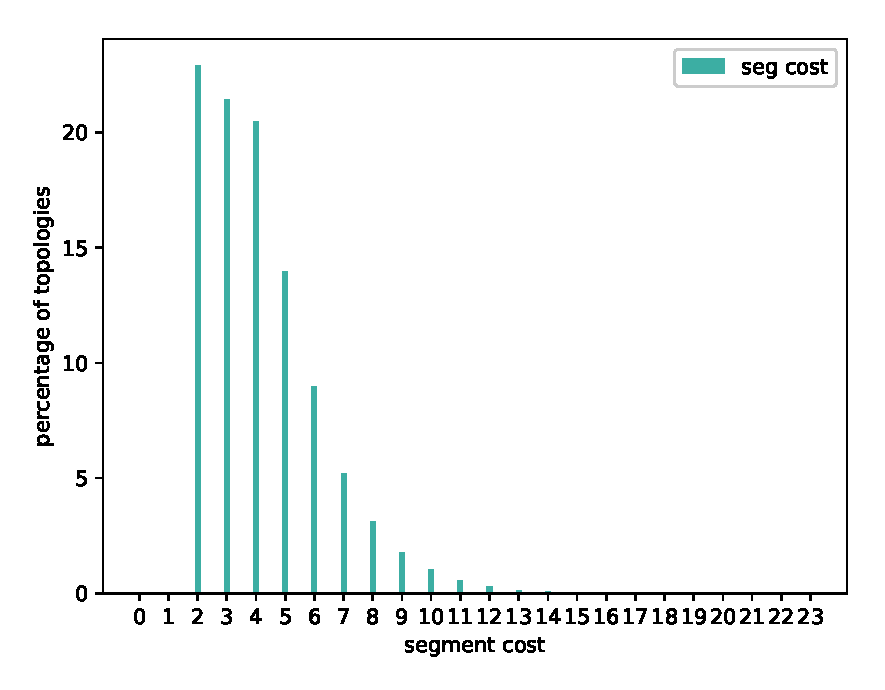
\includegraphics[width=.85\columnwidth]{./Network-lib/data/plot/minCostEDP_segcost.eps}
\end{center}
\caption{Distribution of the maximum segment of maximum cardinality sets of disjoint paths with total minimum latency.}
\label{fig:minCostEDP_segcost}
\end{figure}

\subsection{Maximum set of disjoint sr-paths}

We propose two MIP models for adapting the graph model $\maxedp(G, s, t)$ to Problem \ref{prob:max-sr-edp}. We start by defining
an indicator function telling use whether an edge belongs to the shortest paths between two given nodes.
That is, let $I$ to denote a function $V(G)^2 \times E(G) \rightarrow \{0, 1\}$ defined such that $I(u, v, e) = 1$ if and only if $e \in E(\sp(u, v))$.

Our first model is an adaptation of the traffic engineering segment model $\srteseg(G, \mathcal{D})$ proposed in Chapter \ref{chapter:te}. 
Our demand set contains unit demands between $s$ and $t$. Each such demand corresponds to a sr-path that is edge-disjoint from the
others. We can select the number of demands to be equal to the out-degree of $s$, since this is an upper bound on the number
of disjoint paths from $s$ to any other node. Our objective will by to route a maximum
amount of demands in a way such that no two demands are routed over the same edge. We use variables $x^d_{uv}$ 
saying whether $\sp(u, v)$ is used by the sr-path corresponding to demand $d$. We replace the capacity constraints
by disjointness constraints which consists of requiring that for each edge, at most one demand is routed over it. The rest of the model
is the same as $\srteseg(G, \mathcal{D})$ which uses flow constraints to ensure that paths go from $s$ to $t$.

\begin{center}
\begin{tabular}{rcllr}
\multicolumn{5}{l}{$\sredpseg(G, s, t)$} \\[0.5cm] 
\multicolumn{3}{l}{$\mathbf{max} \quad \displaystyle \sum_{u \in V(G)} \sum_{d = 1}^r x^d_{su}$} & $\textbf{s.t.}$ & \\[0.5cm]
%\multicolumn{5}{l}{{\color{gray!80!white} qsdqsd qsdqsaz sqd s dazz azeqsd azee aze qsd }} \\
$\displaystyle \sum_{d = 1}^r \sum_{u \in V(G)} \sum_{v \in V(G)}  x^d_{uv} \cdot I(u, v, e)$ & $\leq$ & $1$ & $\forall e \in E(G)$ & \\[0.5cm]
$\displaystyle \sum_{u \in V(G) \setminus \{ v \}} x^d_{uv} - \sum_{u \in V(G) \setminus \{ v \}} x^d_{vu}$ & $=$    &  $0$ & $\forall d$, & \\[-0.2cm]
& & & $\forall v \in V(G) \setminus \{ s, t \}$ & \\[0.5cm]
$\displaystyle \sum_{d = 1}^r \sum_{u \in V(G) } x^d_{us} + x^d_{tu}$ & $=$    &  $0$ & $\forall d \in \{1, \ldots, |\oute(s)|\}$ \\[0.5cm] 
$\displaystyle \sum_{u \in V(G)} \sum_{v \in V(G)} x^d_{uu}$ & $\leq$    &  $k$ & $\forall d \in \{ 1, \ldots, |\oute(s)| \}$, \\[0.5cm]
$x^d_{uv}$  &    $\in$    &  $\{0, 1\}$  & $\forall e \in E(G),$ & \\
  &    &   & $\forall d \in \{1, \ldots, |\oute(s)|\}$ &
\end{tabular}
\end{center}

Next, we propose another model whose original idea is due to
Bernard Fortz. After we will compare both models. Note that both these models only support node segments
in the sr-paths.

%For simplicity, we start by presenting the model for sr-paths consisting
%only on node segments. We will describe later how to extend it to also take into account
%adjacency segments as well. 
%As it was already observed by Renauld Hartert, a sr-path 
%consisting only on node segments can between seen as a path on the complete graph
%with $V(G)$ nodes. The correspondence is quite clear as a sr-path with only node segments
%is a sequence $\langle x_1, \ldots, x_l \rangle$ such that each $x_i \in V(G)$ and a
%path on the complete graph also is a sequence $(v_1, \ldots, v_r)$ with each $v_i \in V(G)$.
A sr-path with only node segments is a sequence $\langle y_1, \ldots, y_l \rangle$
such that each $y_1, \ldots, y_l \in V(G)$. The idea behind Fortz  model is to define binary variables 
$x^i_{uv}$ such that $x^i_{uv} = 1$ if and only if
$u$ and $v$ appear as consecutive segments $y_i = u$ and $y_{i + 1} = v$ of a sr-path used in the solution.
These variables are defined for $i = 1, \ldots, k - 1$ where $k$ is the maximum segment cost that we
want to allow the paths to have. Consider for instance that we have a solution where
$x^1_{sa} = x^2_{ab} = x^3_{bt} = 1$. This will correspond to using the sr-path $\langle s, a, b, t\rangle$
as shown in Figure \ref{fig:modelfortz}. So, basically, the index $i$ is saying the position at which we use
each segment.
Note that a more intuitive model would be to drop the $i$ index and use variables $x_{uv}$ to mean that we use
the shortest paths between $u$ and $v$ to route traffic. By adding flow conservation constraints similar to the
ones used in model $\maxflow(G, s, t)$ we can make sure that these variables actually come together
to constitute sr-paths. However, this gives no way of restricting the segment cost of those paths.


\begin{figure}
\begin{center}
\begin{tikzpicture}
\draw[gray, dashed] (0, 0) -- (0, 5) node[anchor=south] {$i = 1$};
\draw[gray, dashed] (2, 0) -- (2, 5) node[anchor=south] {$i = 2$};
\draw[gray, dashed] (4, 0) -- (4, 5) node[anchor=south] {$i = 3$};
\draw[gray, dashed] (6, 0) -- (6, 5) node[anchor=south] {$i = 4$};
\node[scale=0.15] (s) at (-1, 2.5) {\router{s}{router}};
\node[scale=0.15] (a) at (1, 4) {\router{$a$}{router}};
\node[scale=0.15] (b) at (3, 3.5) {\router{$b$}{router}};
\node[scale=0.15] (t1) at (5, 3.75) {\router{$t$}{router}};

\node[scale=0.15] (c) at (1, 5 - 4 - 0.5) {\router{$c$}{router}};
\node[scale=0.15] (d) at (3, 5 - 3.5 - 0.5) {\router{$d$}{router}};
\node[scale=0.15] (e) at (5, 5 - 3.75 - 0.5) {\router{$e$}{router}};
\node[scale=0.15] (t2) at (7, 2.5) {\router{$t$}{router}};


\draw (s) edge[line width=2, above, sloped, ->] node {\small $x^1_{s a} = 1$} (a);
\draw (a) edge[line width=2, above, sloped, ->] node {\small $x^2_{a b} = 1$} (b);
\draw (b) edge[line width=2, above, sloped, ->] node {\small $x^3_{b t} = 1$} (t1);

\draw (s) edge[line width=2, above, sloped, ->] node {\small $x^1_{s c} = 1$} (c);
\draw (c) edge[line width=2, above, sloped, ->] node {\small $x^2_{c d} = 1$} (d);
\draw (d) edge[line width=2, above, sloped, ->] node {\small $x^3_{d e} = 1$} (e);
\draw (e) edge[line width=2, above, sloped, ->] node {\small $x^4_{e t} = 1$} (t2);

\node[right = 0.1cm of t2] {$\langle s, c, d, e, t \rangle$};
\node[right = 0.1cm of t1] {$\langle s, a, b, t \rangle$};
\end{tikzpicture}
\end{center}
\caption{Two examples of how the variables $x^i_{uv}$ define sr-paths.}
\label{fig:modelfortz}
\end{figure}

\begin{center}
\begin{tabular}{crcllr}
\multicolumn{5}{l}{$\sredpfortz(G, s, t)$} \\[0.5cm] 
$\displaystyle \mathbf{max}$ & $\displaystyle \sum_{u \in V(G)} x^1_{su}$ & & & & \\[0.5cm]
$\textbf{s.t.}$ & $\displaystyle \sum_{i = 1}^k \sum_{u \in V(G)} \sum_{v \in V(G)} I(u, v, e) \cdot x^i_{uv} $ & $\leq$    & $1$ & $\forall e \in E(G)$  & $(1)$ \\[0.5cm]
                & $\displaystyle \sum_{v \in V(G)} x^{i - 1}_{vu} - \sum_{v \in V(G)} x^i_{uv}$ & $=$ & $0$ & $\forall u \in V(G) \setminus \{s, t\}$, &  $(2)$ \\[-0.2cm] 
                & & & & $i = 2, \ldots, k$ &  \\[0.5cm] 
                & $\displaystyle \sum_{i = 1}^k \sum_{v \in V(G)} x^i_{vs} + x^i_{tv}$ & $=$ & $0$ &  & $(3)$ \\[0.5cm]
                & $\displaystyle \sum_{v \in V(G) \setminus \{s\}} x^1_{vu} + \sum_{v \in V(G) \setminus \{t\}} x^k_{uv}$ & $=$ & $0$ & $\forall u \in V(G)$ & $(4)$\\[0.5cm]
                & $x_{e}$ & $\in$ & $\mathbb{N}$
\end{tabular}
\end{center}

Constraints $(1)$ ensure that each edge is used only once making sure that the final paths are indeed edge-disjoint. Recall that setting $x^{i - 1}_{uv}$ to $1$ means that
node $u$ is used as a node segment at position $i - 1$ in some sr-path in the solution. Thus, if $u \neq t$ we need to make sure that there is also some node $v'$ coming after $u$ in this sr-path as
illustrated in Figure \ref{fig:modelfortz2}. This is what constraints $(2)$ ensure, that is, that for each $u$ such that $x^{i - 1}_{vu}$ for some $v$, there is also some element
$v'$ such that $x^{i}_{uv'}$ ensuring that the path does not end at a node $u \neq t$. 
These constraints are similar to the classical conservation constraints that are commonly used in these kinds of models to ensure connectivity.



\begin{figure}
\begin{center}
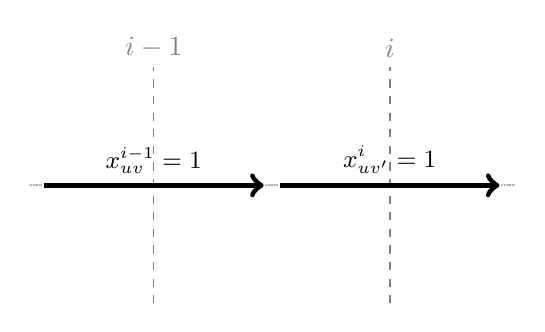
\begin{tikzpicture}
\draw[gray, dashed] (1, 1) -- (1, 4) node[anchor=south] {$i - 1$};
\draw[gray, dashed] (4, 1) -- (4, 4) node[anchor=south] {$i$};
\node[scale=0.15] (v) at (-0.5, 2.5) {\router{$v$}{router}};
\node[scale=0.15] (u) at (2.5, 2.5) {\router{$u$}{router}};
\node[scale=0.15] (v2) at (5.5, 2.5) {\router{$v'$}{router}};

\draw (v) edge[line width=2, above, sloped, ->] node {\small $x^{i - 1}_{uv} = 1$} (u);
\draw (u) edge[line width=2, above, sloped, ->] node {\small $x^{i}_{uv'} = 1$} (v2);

\end{tikzpicture}
\end{center}
\caption{If $x^{i - 1}_{uv} = 1$ .}
\label{fig:modelfortz2}
\end{figure}

Constraints $(3)$ simply make sure that $s$ appears only as the first element of the sr-paths and that $t$ occurs only as the last one.
Finally, constraints $(4)$ prevent other nodes to be the starting and end-points of paths by ensuring that $x^1_{uv}$ can only be set if $u = s$
and that $x^k_{uv}$ can only be set if $v = t$.

Figure \label{fig:maxEDP_runtime} shows a CDF of the runtime needed to compute optimal solutions of $\sredpseg(G, s, t)$  and $\sredpfortz(G, s, t)$ using Gurobi. In
both cases the maximum number of segments was set to $5$. We generated
$100$ random source-destination pairs and solved both models over these pairs for all instances in our dataset. We can see (in orange) that the segment
model is slower than the model proposed by Fortz (in blue). We see that the maximum runtime of the Fortz model is about $3$ minutes whereas
the maximum runtime of the segment model is about $10$ minutes. In both cases this shows that using a MIP solver for computing sets of disjoint
sr-paths is feasible in practice in a reasonable amount of time. 
In order to try to understand whether our sample of $100$ pairs is large enough, we computed a box-plot of the run times on the topologies from groups
\texttt{real} and \texttt{rf} of the Fortz model. 
We selected these because they are the largest ones and we cannot show all results in the box plot. Figure \ref{fig:maxEDP_boxplot} shows these. Except for
topology \texttt{1239}, the runtime does not have a high variance so we can expect that the average runtime is close
to the one computed.

\begin{figure}
\begin{center}
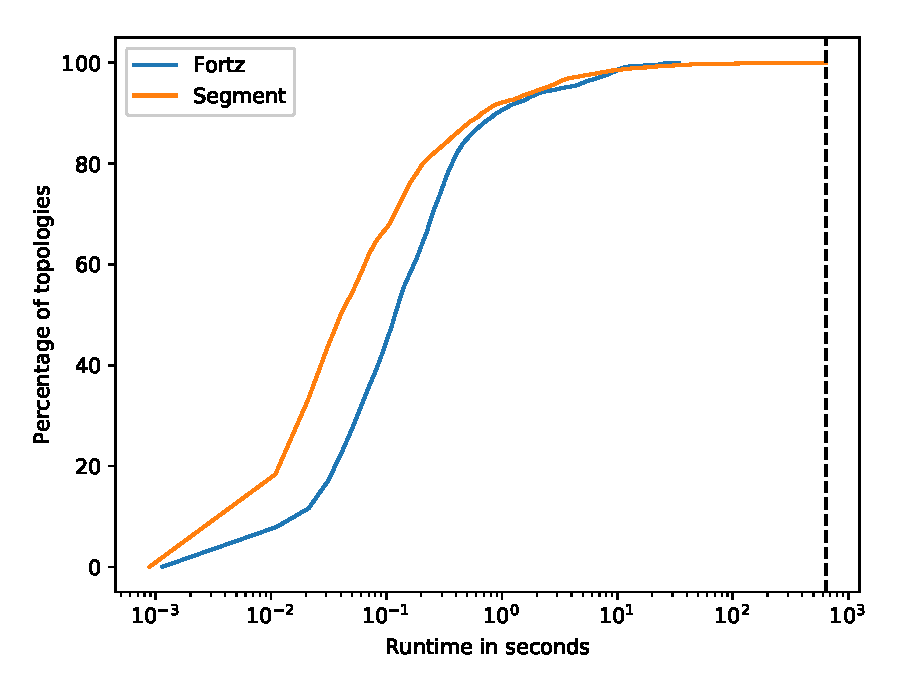
\includegraphics[width=.85\columnwidth]{./Network-lib/data/plot/maxEDPMip_runtime_both.eps}
\end{center}
\caption{CDF over all topologies of the runtime for solving $\sredpseg(G, s, t)$ and $\sredpfortz(G, s, t)$ over $100$ randomly selected source-destination pairs.}
\label{fig:maxEDP_runtime}
\end{figure}

\begin{figure}
\begin{center}
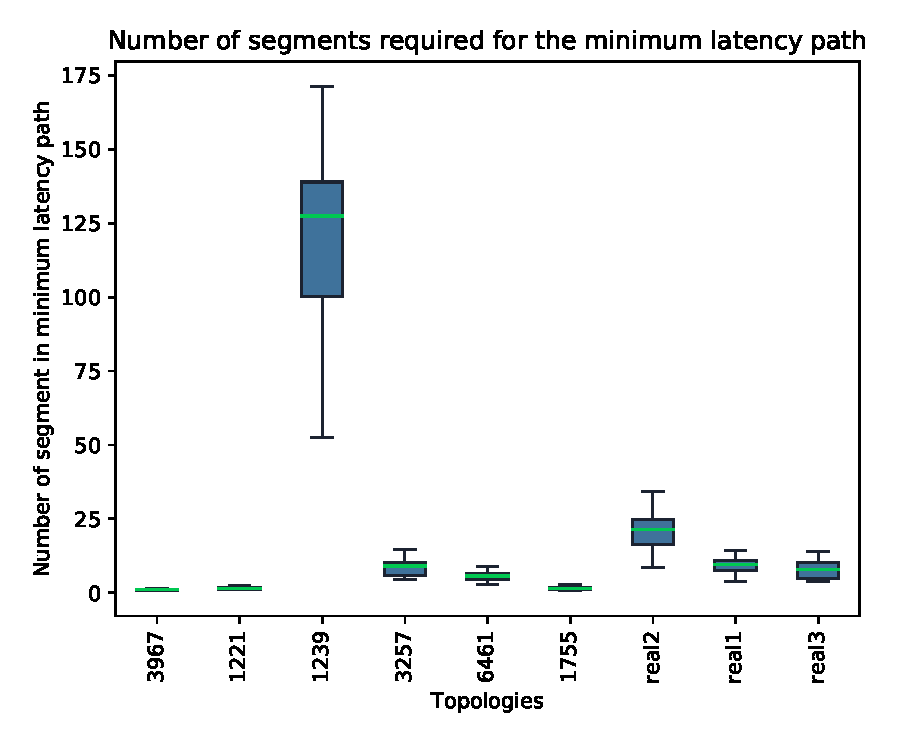
\includegraphics[width=.85\columnwidth]{./Network-lib/data/plot/maxEDP_boxplot.eps}
\end{center}
\caption{CDF over all topologies of the runtime for solving $\sredpfortz(G, s, t)$ over $100$ randomly selected source-destination pairs.}
\label{fig:maxEDP_boxplot}
\end{figure}

We also analyzed how restrictive the segmentation constraints with respect to the existence of disjoint paths.
For this we computed the difference between the maximum number of disjoint paths between the sources and the destinations
with the maximum number of disjoint sr-paths of segment cost at most $5$. Whenever this difference is $0$ we know that
requiring the path to be implementable with a segment cost of at most $5$ posed no restrictions in finding solutions.
Table \ref{tab:nbp_vs_seg} shows these results. We can see that for $95\%$ of the pairs the segmentation constraints were
not restrictive. This indicates that with about $5$ segments we can implement sets of sr-paths that are as large as the
theoretical maximum supported on the graph topology.

\begin{figure}
\begin{center}
\begin{tabular}{rccccc}
\toprule
difference & $0$ & $1$ & $2$ & $3$ & $\geq 4$ \\
\midrule
percentage of $s$-$t$           & 95\% & 4\% & 0.4\% & 0.1\% & 0.5\%
\end{tabular}
\end{center}
\caption{Percentage of pairs for each value of the difference between the maximum number of disjoint paths and maximum number of disjoint sr-paths with segment
cost at most $5$.}
\label{tab:nbp_vs_seg}
\end{figure}

\subsection{Minimizing the total latency}

For both models it is straightforward to modify the models to minimize the total latency of the sr-paths.
In both cases we need to first compute the maximum number of disjoint sr-paths that exist between the source
and destination, say $P$. Then, we need to replace the objective function by a minimization function that
adds all latencies together. We also need an additional constraint requiring the total number of paths in the solution to be equal to $P$.
Concretely, in the segment model, $\sredpseg(G, s, t)$, we can obtain this by replacing the objective function by
$$
\textbf{minimize} \quad \sum_{d = 1}^r \sum_{u \in V(G)} \sum_{v \in V(G)} \lat(u, v) \cdot x^d_{uv} 
$$
and adding a constraint
$$
\sum_{u \in V(G)} \sum_{d = 1}^r x^d_{su} = P. 
$$
For the Fortz model, $\sredpfortz(G, s, t)$, the change is analogous. The objective function
becomes 
$$
\textbf{minimize} \quad \sum_{i = 1}^k \sum_{u \in V(G)} \sum_{v \in V(G)} \lat(u, v) \cdot x^i_{uv} 
$$
and we add a constraint requesting $P$ paths starting at the source $s$:
$$
\sum_{u \in V(G)} x^1_{su} = P. 
$$

%\todo{Add plot comparing the runtime of minimizing latency vs not.}

\section{Min-max edge-disjoint sr-paths}

We now focus on the problem of computing pairs of disjoint paths with a min-max objective function. More
specifically, we aim at connecting via disjoint sr-paths a source node 
$s_1$ to a destination $t_1$ and a source node $s_2$ to a destination $t_2$
such that the maximum latency among those two paths is as small as possible.

\begin{problem}{Min-max edge-disjoint sr-paths}
\label{prob:disjointsrp}
\textbf{Input:} A network $G$ and $s_1, s_2, t_1, t_2 \in V(G)$ such that $s_1 \neq t_1$ and $s_2 \neq t_2$
and $k \in \mathbb{N}$.

\textbf{Output:} Two disjoint sr-paths $\sr{p}_1 \in \Pk(s_1, t_1), \sr{p}_2 \in \Pk(s_2, t_2)$ such that
$$
\max (\lat(\sr{p}_1), \lat(\sr{p}_2))
$$
is minimal.
\end{problem}

As we mentioned in the previous section, this problem is \NPhard \cite{minmax-disjoint-90, Li1990}.

\subsection{MIP formulation}

We saw above that Fortz model performed better than the segment model for computing maximal sets of disjoint paths.
However it is hard to enforce a source to destination assignment with this model. The reason is that different paths are not
modeled explicitly. For this reason, we use the segment model for solving Problem \ref{prob:disjointsrp}. With the segment model
each path is encoded in the index $d$ of the variables $x^d_{uv}$. This makes it easy to for the path starting at $s_1$ to end at $t_1$ and the
path starting at $s_2$ to end at $t_2$. The adapted model is the following.

\begin{center}
\begin{tabular}{rcllr}
\multicolumn{5}{l}{$\sredp(G, s_1, s_2, t_1, t_2)$} \\[0.5cm] 
\multicolumn{3}{l}{$\mathbf{min} \quad \lambda$} & $\textbf{s.t.}$ & \\[0.5cm]
$\displaystyle \sum_{d = 1}^2 \sum_{u \in V(G)} \sum_{v \in V(G)}  x^d_{uv} \cdot I(u, v, e)$ & $\leq$ & $1$ & $\forall e \in E(G)$ & \\[0.5cm]
$\displaystyle \sum_{u \in V(G) \setminus \{ v \}} x^d_{uv} - \sum_{u \in V(G) \setminus \{ v \}} x^d_{vu}$ & $=$    &  $0$ & $\forall d \in \{1,2\}$, $\forall v \in V(G) \setminus \{ s_d, t_d \}$ & \\[0.5cm]
$\displaystyle \sum_{u \in V(G)} \sum_{v \in V(G)} \lat(u, v) \cdot x^d_{u, v}$ & $\leq$    & $\lambda$ & $\forall d \in \{ 1, 2 \}$ \\[0.5cm]
$\displaystyle \sum_{u \in V(G) \setminus \{ s_d \}} x^d_{s_d u}$ & $=$    & $1$ & $\forall d \in \{ 1, 2 \}$ \\[0.5cm]
$\displaystyle \sum_{u \in V(G) \setminus \{ t_d \}} x^d_{u t_d}$ & $=$    & $1$ & $\forall d \in \{ 1, 2 \}$ \\[0.5cm]
$\displaystyle \sum_{d = 1}^2 \sum_{u \in V(G)} x^d_{u s_d} +  x^d_{t_d u}$ & $=$    & $0$ & $\forall d \in \{ 1, 2 \}$ \\[0.5cm]
$\displaystyle \sum_{u \in V(G)} \sum_{v \in V(G)} x^d_{uu}$ & $\leq$      & $k$ & $\forall d \in \{ 1, 2 \}$ \\[0.5cm]
$x^d_{uv}$  &    $\in$    &  $\{0, 1\}$  & $\forall e \in E(G), \ \forall d \in \{1, 2 \}$ & \\[0.5cm]
$\lambda$   &    $\geq$   & $0$ & &
\end{tabular}
\end{center}


\subsection{Dedicated algorithm}

We also proposed a dedicated algorithm for solving this problem. This was actually our original idea that was published in CoNEXT 18 \cite{rdp}.
However we will see that it is actually less efficient and flexible than the MIP formulation.
Recall that in our definition of network, we mentioned that each edge is indexed with a unique number between $0$ and $|E(G)| - 1$. This is useful for
defining parallel edges. These indexes are also important in the context of disjoint paths. From an implementation point of view, we will represent the
set of edges corresponding to a sr-path $\sr{p}$, $E(\sr{p})$, as a \emph{bitset} $b$ such that $b_i = 1$ if and only if edge with $\idx(e) = i$ belongs
to $E(\sr{p})$.

Bitsets are a very simple and efficient way to represent subsets of $\{ 0, \ldots, n - 1 \}$ for some fixed, not too large value of $n$. Conceptually they
are similar to an array of booleans of size $n$. However, a bitset is represented instead (on a 64-bit machine) with an array of \texttt{long}. Each element of the array
represents a group of $64$ boolean values with its bits. So the bits of the first element in the array will represent elements $0$ to $63$, the second $64$ to $127$ and 
so forth. Figure \ref{fig:bitset} illustrates a bitset for $n = 512$. In this example, element $131$ is represented by the forth bit of
the third long.

\begin{figure}
\begin{center}
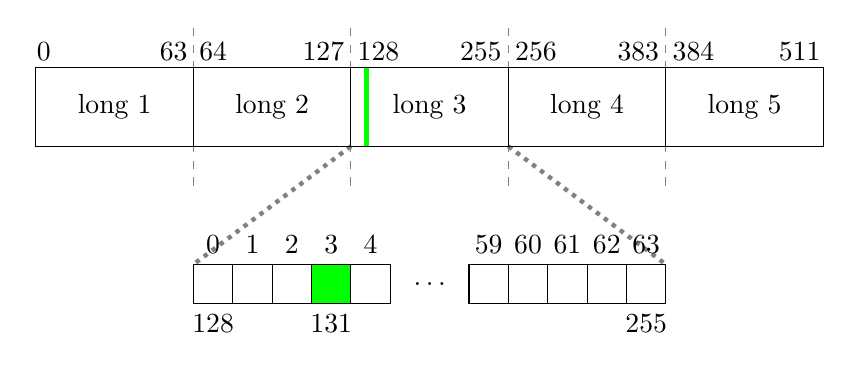
\begin{tikzpicture}

\draw[green, ultra thick] (4.2, 0) -- (4.2, 1);


\draw[dashed, gray] (2, -0.5) -- (2, 1.5);
\draw[dashed, gray] (4, -0.5) -- (4, 1.5);
\draw[dashed, gray] (6, -0.5) -- (6, 1.5);
\draw[dashed, gray] (8, -0.5) -- (8, 1.5);

\fill[green] (3.5, -2) rectangle (4, -1.5);

\draw[gray, ultra thick, dotted] (4, 0) -- (2, -1.5);
\draw[gray, ultra thick, dotted] (6, 0) -- (8, -1.5);

\draw[step=2] (0, 0) grid (10, 1);
\draw (0, 0) rectangle (10, 1);

\draw[step=0.5] (2, -2) grid (4.5, -1.5);
\draw (2, -2) rectangle (4.5, -1.5);

\draw[step=0.5] (5.5, -2) grid (8, -1.5);
\draw (5.5, -2) rectangle (8, -1.5);

\node at (5, -1.75) {$\ldots$};

\node at (2.25, -1.25) {0};
\node at (2.75, -1.25) {1};
\node at (3.25, -1.25) {2};
\node at (3.75, -1.25) {3};
\node at (4.25, -1.25) {4};


\node at (2.25, -2.25) {128};
\node at (2.25 + 1.5, -2.25) {131};

\node at (5.5 + 2.25, -2.25) {255};

\node at (5.5 + 0.25, -1.25) {59};
\node at (5.5 + 0.75, -1.25) {60};
\node at (5.5 + 1.25, -1.25) {61};
\node at (5.5 + 1.75, -1.25) {62};
\node at (5.5 + 2.25, -1.25) {63};

\node at (0.1, 1.2) {0};
\node at (1.75, 1.2) {63};

\node at (2.25, 1.2) {64};
\node at (3.65, 1.2) {127};

\node at (4.35, 1.2) {128};
\node at (5.65, 1.2)  {255};

\node at (6.35, 1.2) {256};
\node at (7.65, 1.2) {383};

\node at (8.35, 1.2) {384};
\node at (9.7, 1.2) {511};

\node at (1, 0.5) {long 1};
\node at (3, 0.5) {long 2};
\node at (5, 0.5) {long 3};
\node at (7, 0.5) {long 4};
\node at (9, 0.5) {long 5};

\end{tikzpicture}
\end{center}
\caption{Representation of a bitset with $n = 512$.}
\label{fig:bitset}
\end{figure}

The advantage of this representation over a boolean array representation is that each set operation on a long can be performed in $O(1)$.
So for example, to compute the intersection between two bitsets we simply need to loop over the array and perform a bitwise and between
corresponding elements. Therefore we only need to perform $n \slash 64$ operations rather $n$. Even though in big-Oh notation this sill yields
the same complexity, $O(n)$, the runtime in practice is $64$ times faster which is a gigantic speedup.
Using a bitset representation for the set of edges of a sr-path we can then perform set operations over these very efficiently. 

In particular, this representation makes it possible to very efficiently check whether or not two sr-paths are disjoint. We exploit this to
design an algorithm for solving \ref{prob:disjointsrp}. Given a sr-path $\sr{p}_1$ we can find the minimum latency sr-path $\sr{p}_2$ that
is disjoint from it in polynomial time by using the minimum latency sr-path algorithm from Chapter \ref{chapter:sr-optimal}. We simply need to
adapt it so that it avoids $E(\sr{p}_1)$. To do so, we need to know the set of edges in all sr-paths of the form $\langle x, y \rangle$
where $x, y \in V(G)$. We show how to do this in the next.

\subsubsection{Pre-computing the forwarding graphs}

\begin{lemma}
\label{lemma:forwdp}
Let $G$ be a network and $x, y \in V(G)$. Then
\begin{equation}
\label{eq:forwdp}
E(\sp(x, y)) = \bigcup_{ e \in \ine(\sp(x), y) } E(\sp(x, e^1)) \cup \{ e \}.
\end{equation}
\end{lemma}

\begin{proof}
$(\subseteq)$ Let $e \in E(\sp(x, y))$. Let $p = (e_1, \ldots, e_n)$ be a shortest path from $x$ to $y$ 
passing by $e$. Then $e = e_i$ for some $i$.  Note that $(e_1, \ldots, e_{n - 1})$ 
is a shortest path from $x$ to $e^2_{n - 1} = e^1_n$ and, since $e^2_n = y$, 
$e_n \in \ine(\sp(x), y)$. Thus, if $i = n$ then $e$ clearly belongs to the right-hand
side of (\ref{eq:forwdp}). Otherwise, if $i < n$ then $e$ belongs to the shortest 
path $(e_1, \ldots, e_{n - 1})$ from $x$ to $e^2_{n - 1} = e^1_n$. Since $e_n \in
\ine(\sp(x), y))$ we again conclude that $e$ belongs to the rhs of (\ref{eq:forwdp}).

$(\supseteq)$ Let $e$ be a edge belonging to the rhs of (\ref{eq:forwdp}). There exists
$f \in \ine(\sp(x), y))$ such that either $e = f$ or $e \in E(\sp(x, f^1))$. If $e = f$
then $e = f \in \ine(\sp(x), y)) = \ine(\sp(x, y))$ so it belongs to $\sp(x, y)$. Otherwise,
$e$ belongs to a shortest path from $x$ to the origin of $f$. Since $f \in \ine(\sp(x), y)$
we have that $\dist(x, y) = \dist(x, f^1) + \igp(f)$. Since $e$ belongs to a shortest
path $p$ from $x$ to $f^1$, we have 
$\dist(x, e^1) + \igp(e) + \dist(e^2, f^1) = \dist(x, f^1) = \igp(p)$.
Then
\begin{align*}
\dist(x, y) & = \dist(x, f^1) + \igp(f) \\
& = \dist(x, e^1) + \igp(e) + \dist(e^2, f^1) + \igp(f) \\
& = \dist(x, e^1) + \igp(e) + \dist(e^2, f^2) \\
& = \dist(x, e^1) + \igp(e) + \dist(e^2, y) \\
\end{align*}
so that $e \in \sp(x, y)$.
\end{proof}

Using Lemma \ref{lemma:forwdp} we can leverage the speed of bitsets to
efficiently compute $E(\SP(v, u))$ for all $u, v \in V(G)$. Note that we
could always compute them using the definition, that is, computing 
$\sp(u)$ for all $u$ and then for each $v$ using a breath-first search to
extract the subset of edges of $\sp(u)$ that belong to $\sp(u, v)$. 
Using equation (\ref{eq:forwdp}), we can compute $E(\sp(u, v))$ by
performing $|\ine(\sp(u), v)|$ bitset operations. As we mentioned above,
in theory this is not faster but it practice it runs faster even due to the
usage of bitsets. However, in the next section we will see that applying the same idea
to precompute another kind of data that we will need leads to huge gains in
runtime. Algorithm \ref{algo:preforw} shows how we can easily compute this recurrence.
For each $u$ we compute the shortest path subnetwork rooted at $u$ and then compute
a topological order $v_1, v_2, \ldots, v_n$ to compute $E(\sp(u, v_i)$ in an order such
that when computing $E(\sp(u, v_i))$ we already computed $E(\sp(u, e^1))$ for all $e \in
\ine(\sp(u), v_i)$.

%as shown in Figure \ref{fig:precompute_forw_runtime}.

%\begin{figure}
%\begin{center}
%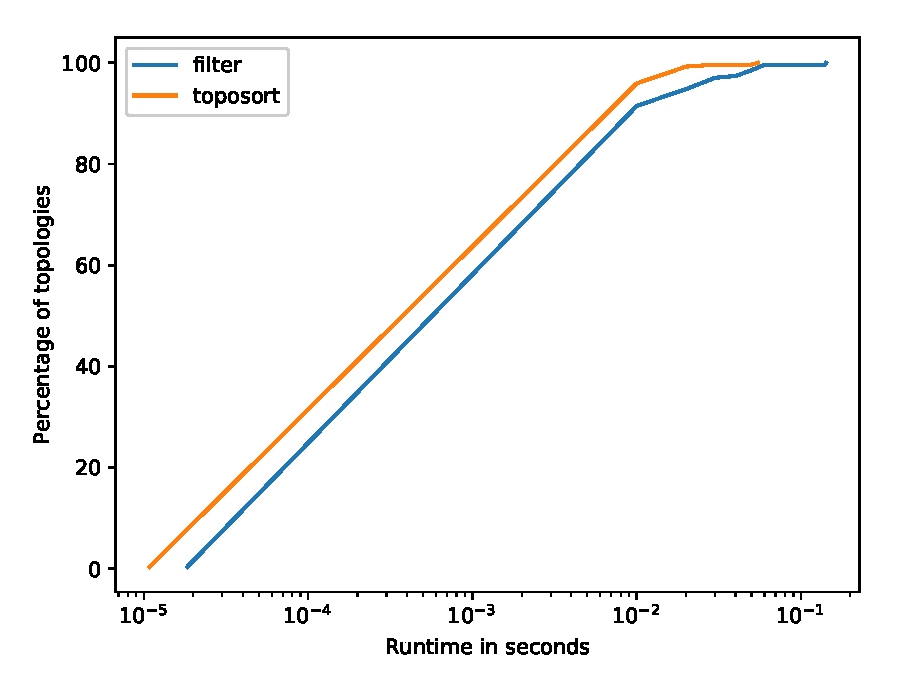
\includegraphics[width=.85\columnwidth]{./Network-lib/data/plot/precompute_forw_runtime.eps}
%\end{center}
%\caption{todo}
%\label{fig:precompute_forw_runtime}
%\end{figure}

\begin{algorithm}[t]
\small
\caption{$\textsf{precompute-forwEdges}\left( g \right)$}
\begin{algorithmic}[1]
\FOR{$u, v \in V(G)$}
  \STATE $fwe(u, v) \gets \textsf{Bitset}()$
\ENDFOR
\FOR{$u \in V(G)$}
  \STATE $\sp(u) \gets \textsf{dikstra-dag}(g, u)$
  \STATE $order \gets \textsf{toposort}(\sp(u))$
  \FOR{$v \in order$}
    \FOR{$e \in \ine(\sp(u), v)$}
      \STATE $fwe(u, v) \gets fwe(u, e^1) \cup \{ e \}$
    \ENDFOR
  \ENDFOR
\ENDFOR
\RETURN $fwe$
\end{algorithmic}
\label{algo:preforw}
\end{algorithm}

Having pre-computed $E(\sp(u, v))$ we can easily adapt Algorithm
\ref{algo:min_weight_sr_path} to make sure that the path that is computed avoids all
edges in $E(\sr{p}_1)$. Recall that, according to Chapter \ref{chapter:sr-optimal}, 
the recurrence for the minimum latency path
from $s_2$ to $v$ with segment cost at most $i$ will be

\[\mathit{sol}(i, v) = \min \left\{
  \begin{matrix}
    \mathit{sol}(i - 1, v) &  \\[0.2cm]
    \mathit{sol}(i - 1, u)  +  \lat(u, v)  & \textbf{s.t} \text{ $u \in V$} \\[0.2cm]
    \mathit{sol}(i - 2, r)  +  \lat(r, e^1) + \lat(e) & \textbf{s.t} \text{ $u \in V, e \in \ine(v)$} \\
\end{matrix}
  \right.
\]

as illustrated by Figure \ref{fig:dp_disjoint}. In order to guarantee disjointness,
we just need to ensure that for each case all pieces are disjoint
from $\sr{p}_1$. This means ensuring that 
$$
E(\sp(u, v)) \cap E(\sr{p}_1) = \emptyset
$$
in the second case and that 
$$\left( E(\sp(u, e^1)) \cup \{ e \} \right) \cap E(\sr{p}_1) = \emptyset
$$
in the third case. In term of algorithms, this corresponds to adding these conditions
to lines \ref{mwsrp-if1} and \ref{mwsrp-if2} from Algorithm \ref{algo:min_weight_sr_path}, respectively. Note that these changes will
have a minor impact over the overall performance of the algorithm since we use bitsets
to compute these intersections and $E(\sp(u, v))$ is given as input for all $u, v \in V(G)$.

 \begin{figure}
 \begin{center}
 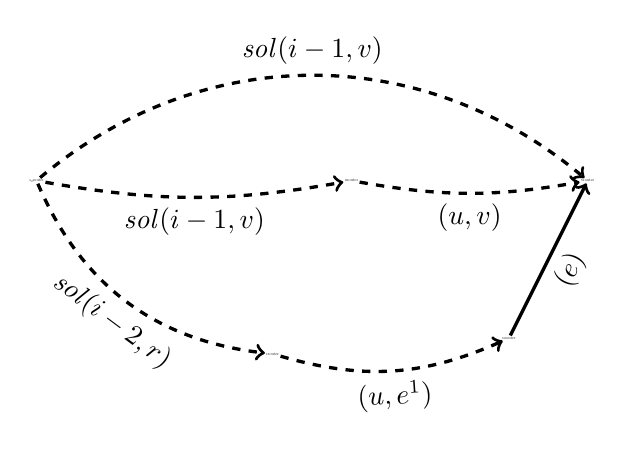
\begin{tikzpicture}
 \node[scale=0.15] (s) at (0, 0) {\router{$s_2$}{router}};
 \node[scale=0.15] (x) at (5+2, 0) {\router{v}{router}};
 \node[scale=0.15] (y) at (2+2, 0) {\router{u}{router}};
 \node[scale=0.15] (z) at (4+2, -2) {\router{u}{router}};
 \node[scale=0.15] (r) at (2+1, -2-0.2) {\router{r}{router}};
 
 
 
 \draw (s) edge[very thick, below, bend right=10, dashed, ->] node {$\mathit{sol}(i - 1, v)$} (y);
 \draw (y) edge[very thick, bend right=10, dashed, ->, below] node {$\lat(u, v)$} (x);
 \draw (s) edge[very thick, bend left=40, dashed, ->, above] node {$\mathit{sol}(i - 1, v)$} (x);
 %\draw (s) edge[very thick, bend right=30, dashed, ->] (z);
 \draw (z) edge[very thick, ->, sloped, below] node {$\lat(e)$} (x);
 
 \draw (s) edge[very thick, bend right=30, dashed, ->, below, sloped] node {$\mathit{sol}(i - 2, r)$} (r);
 \draw (r) edge[very thick, bend right=20, dashed, ->, below, sloped] node {$\lat(u, e^1)$} (z);
 
 \end{tikzpicture}
 \end{center}
 \caption{Illustration of the $\mathit{sol}$ recurrence}
 \label{fig:dp_disjoint}
 \end{figure}

In order to find a pair of paths, we perform a depth-first search on $\sr{p}_1$ and use
the above algorithm to maintain the minimum latency sr-path $\sr{p}_2$ that is disjoint from the 
current partial path $\sr{p}_1$. At each step of the search, we try to extend $\sr{p}_1$
with either a node segment or an adjacency segment. We perform the following steps to
avoid exploring useless extensions of $\sr{p}_1$. Let $\sr{p}_1 = \langle
x_1, \ldots, x_n \rangle$ be the partial path at given search node, $\sr{p}_2$
the minimum latency sr-path disjoint from the partial path $\sr{p}_1$, $l^*$ the 
latency of the best solution found so far and $x$ be a node or adjacency segment:

\begin{itemize}
 \item Let $v = x^2_n$ be the node where $\sr{p}_1$ ends. In the best case, the latency
 of the completed sr-path $\sr{p}_1$ will be its current latency plus the latency of the minimum
 latency path between $v$ and $t_1$ in $G$. Let's denote that latency by $\mathcal{L}(v, t_1)$.
 Therefore, if $\max(\lat(\sr{p}_1) + \mathcal{L}(v, t_1), \lat(\sr{p}_2)) \geq l^*$
 we can stop the search since we will never reach a better solution.
 
 \item By Theorem \ref{thm:sracyclic}, there is
 a solution to Problem \ref{prob:disjointsrp} where both $\sr{p}_1$ and $\sr{p}_2$ are acyclic.
 Hence, we can ignore $x$ if $\sr{p}_1 \oplus x$ is cyclic. Checking this can be 
 done efficiently thanks to our bitset representation and forwarding graph
 edge set pre-computation.
 
 \item If $\sr{p}_1 \oplus x$ does not intersect 
 $\sr{p}_2$ then $\sr{p}_2$ remains the minimum latency sr-path that is disjoint from
 $\sr{p}_1 \oplus x$ so there is not need to re-compute it. Otherwise, we use the algorithm
 that we described above to compute a new minimum latency sr-path $\sr{p}_2$. If this path does
 not exist, then it is fruitless to try $x$ as an extension of $\sr{p}_1$.
 
 \item If there does not exist a pair of disjoint paths
 on $G$, one from $x^2$ to $t_1$ and another from $s_2$ to $t_2$ then we will never reach a 
 solution by extending $\sr{p}_1$ with $x$. However, we have seen that checking whether
 such disjoint paths exists is \NPcomplete. We use a relaxation of this condition by allowing
 the path from $x^2$ to go to $t_2$ or the path from $s_2$ to go to $t_1$ which is equivalent
 to checking whether the maximum flow between $\{x^2, s_2\}$ and $\{t_1, t_2\}$ is
 at least $2$.
\end{itemize}

By putting all these ideas together we can formally express Algorithm
\ref{algo:disjoint_srp} and \ref{algo:disjoint_srp_dfs} for solving Problem
\ref{prob:disjointsrp}.

\begin{algorithm}[t]
\small
\caption{$\textsf{disjoint-srpaths}\left( g, s_1, s_2, t_1, t_2 \right)$}
\begin{algorithmic}[1]
\STATE $\sr{p}_2 \gets \textsf{min-lat-disjoint-srpath}(s_2, t_2, k)$
\STATE $l^* \gets \infty$
\FOR{$x \in V(G) \cup E(g)$}
  \STATE $\textsf{disjoint-srpaths-dfs}\left( \langle x \rangle, \sr{p}_2 \right)$
\ENDFOR
\IF{$l^* = \infty$}
  \RETURN \textbf{null}
\ENDIF
\RETURN $\sr{p}^*_1, \sr{p}^*_2$
\end{algorithmic}
\label{algo:disjoint_srp}
\end{algorithm}

\begin{algorithm}[t]
\small
\caption{$\textsf{disjoint-srpaths-dfs}\left( \sr{p}_1, \sr{p}_2 \right)$}
\begin{algorithmic}[1]
\IF{$\max(\lat(\sr{p}_1) + \mathcal{L}(\sr{p}_1.\textsf{dest}(), t_1) \geq l^*$} 
  \RETURN
\ENDIF
\cmtline{we reached here so if the path is complete, it is a better solution}
\IF{$\sr{p}_1.\textsf{dest}() = t_1$}
  \STATE $l^* \gets \max(\lat(\sr{p}_1), \lat(\sr{p}_2))$
  \STATE $\sr{p}^*_1, \sr{p}^*_2 \gets \sr{p}_1, \sr{p}_2$
  \RETURN
\ENDIF
\cmtline{try extend $\sr{p}_1$ with a node segment}
\IF{$\cost(\sr{p}_1) + 1 > k$}
  \RETURN
\ENDIF
\FOR{$u \in V(G)$}
  \cmtline{check whether we can cut with min cost flow}
  \STATE $P, l \gets \textsf{min-cost-flow}(g, \{u, s_2\}, \{t_1, t_2\})$
  \IF{$|P| < 2 \textbf{ or } l \geq l^*$}
    \RETURN
  \ENDIF
  \cmtline{check whether adding $u$ will keep $\sr{p}_1$ acyclic}
  \IF{$E(\sp(\sr{p}_1.\textsf{dest}(), u)) \cap E(\sr{p}_1) = \emptyset$}
    \RETURN
  \ENDIF
  \STATE $\sr{p}_1.\textsf{addLast}(u)$
  \IF{$E(\sr{p}_1) \cap E(\sr{p}_2) = \emptyset$}
    \STATE $\textsf{disjoint-srpaths-dfs}\left( \sr{p}_1, \sr{p}_2 \right)$
  \ELSE
    \STATE $\sr{p}'_2 \gets \textsf{min-lat-disjoint-srpath}(\sr{p}_1, s_2, t_2, k)$
    \IF{$\sr{p}'_2 \neq \textbf{null}$}
      \STATE $\textsf{disjoint-srpaths-dfs}\left( \sr{p}_1, \sr{p}'_2 \right)$
    \ENDIF
  \ENDIF
  \STATE $\sr{p}_1.\textsf{removeLast}()$
\ENDFOR
\cmtline{try extend $\sr{p}_1$ with an adjacency segment}
\IF{$\cost(\sr{p}_1) + 2 > k$}
  \RETURN
\ENDIF
\FOR{$e \in E(g)$}
  \cmtline{check whether we can cut with min cost flow}
  \STATE $P, l \gets \textsf{min-cost-flow}(g, \{e^2, s_2\}, \{t_1, t_2\})$
  \IF{$|P| < 2 \textbf{ or } l \geq l^*$}
    \RETURN
  \ENDIF
  \IF{$\left( E(\sp(\sr{p}_1.\textsf{dest}(), e^1)) \cup \{e\} \right) \cap E(\sr{p}_1) \neq \emptyset$}
    \RETURN
  \ENDIF
  \cmtline{check whether adding $e$ will keep $\sr{p}_1$ acyclic}
  \STATE $\sr{p}_1.\textsf{addLast}(e)$
  \IF{$E(\sr{p}_1) \cap E(\sr{p}_2) = \emptyset$}
    \STATE $\textsf{disjoint-srpaths-dfs}\left( \sr{p}_1, \sr{p}_2 \right)$
  \ELSE
    \STATE $\sr{p}'_2 \gets \textsf{min-lat-disjoint-srpath}(\sr{p}_1, s_2, t_2, k)$
    \IF{$\sr{p}'_2 \neq \textbf{null}$}
      \STATE $\textsf{disjoint-srpaths-dfs}\left( \sr{p}_1, \sr{p}'_2 \right)$
    \ENDIF
  \ENDIF
\ENDFOR
\end{algorithmic}
\label{algo:disjoint_srp_dfs}
\end{algorithm}

\subsubsection{Algorithm comparison}

We compared both algorithms in terms of runtime. For this, we generated $100$ tuples
$(s_1, s_2, t_1, t_2)$ and computed disjoint sr-path using the MIP algorithm and the dedicated
algorithm for $k = 3$ and $k = 4$. Figure \ref{fig:perf3} shows the performance profile of the algorithms for $k = 3$.
A performance profile shows the CDF of the ratio of the runtime of each algorithm and the minimum runtime amongst the two.
We can observe that the MIP model is faster for $64\%$ of the tuples. The MIP model is at most
$20$ times slower whereas the dedicated algorithm can be up to $53$ times slower. This 
indicates that MIP model is more efficient than the dedicated algorithm. This gets
even more evident as we grow $k$. For $k = 4$, as shown in Figure \ref{fig:perf4},
the MIP model performs much better than the dedicated algorithm. It is faster for $80\%$
of the tuples and when it is not, it is barely slower.

\begin{figure}
\begin{center}
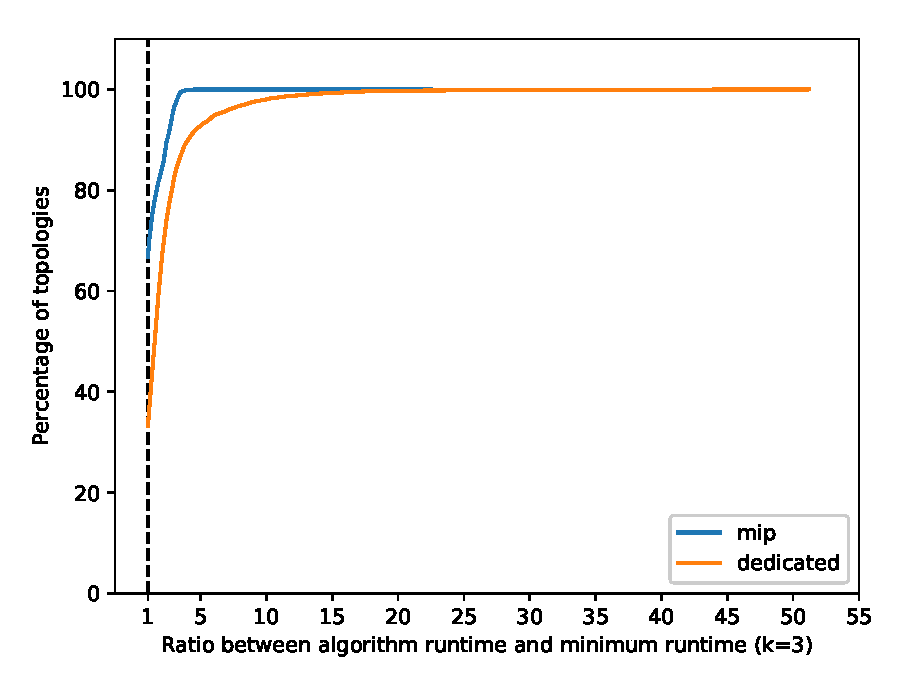
\includegraphics[width=.85\columnwidth]{./Network-lib/data/plot/2SREDP_3.eps}
\end{center}
\caption{Performance profile between the MIP model and the dedicated algorithm for $k = 3$.}
\label{fig:perf3}
\end{figure}

\begin{figure}
\begin{center}
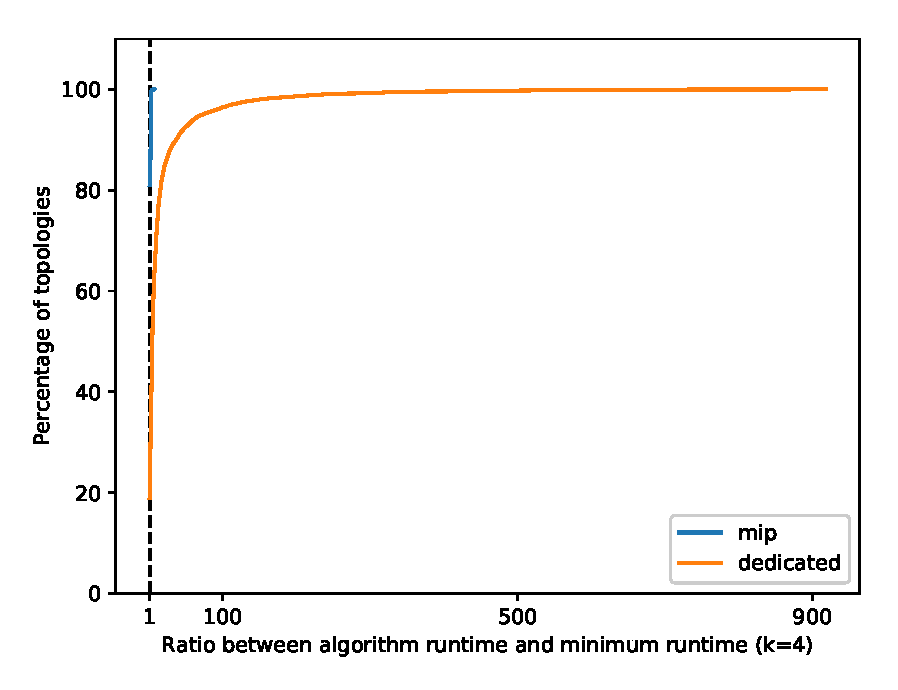
\includegraphics[width=.85\columnwidth]{./Network-lib/data/plot/2SREDP_4.eps}
\end{center}
\caption{Performance profile between the MIP model and the dedicated algorithm for $k = 4$.}
\label{fig:perf4}
\end{figure}



